\documentclass{article}
\usepackage{graphicx}
\usepackage{float}
\usepackage{amsmath}
\begin{document}
	\title{Resum}
	\author{Adrià Bravo Vidal}
	\date{28/04/20}
	\maketitle	
	
Aquesta setmana m'he dedicat, sobretot, a resoldre un gran problema amb el mètode numèric i a acabar de fer comprovacions numèriques de la seva convergència.

\section{Solució d'errors}

Per continuar amb la comporvació de la convergència del mètode, vaig aplicar-hi el problema de l'oscil·lador harmònic. L'oscil·lador harmònic té solució analítica en MQ i podia comparar-hi la evolució de un autoestat aplicant-hi el meu mètode i la analítica. Vam escollir l'estat fonamental, és a dir,
\(nx,ny=0\) per simplicitat. El problema, llavors, es presenta així:

L'estat fonamental:
\begin{equation}
\phi_w(x,y)=\sqrt{\frac{\omega m}{\hbar\pi}}e^{-\frac{m\omega}{2\hbar}(x^2 +y^2)}
\end{equation}

El potencial així:
\begin{equation}
V_w=\frac{1}{2}m\omega^2(X^2+Y^2)
\end{equation}

Energia potencial, cinètica i total:

\begin{equation}
E=\hbar\omega, \quad E_c=\frac{\hbar\omega}{2}, \quad E_p=\frac{\hbar\omega}{2}
\end{equation}

Un cop vam tenir clar quin era el marc de l'oscil·lador harmònic, vam calcular la energia potencial i cinètica del paquet discretitzat en la nostra caixa de a=2L utilitzat un mètode computacional i vam comparar-ho amb l'original. D'aquesta manera vam obtenir figures com aquesta:

\begin{figure}[H]
	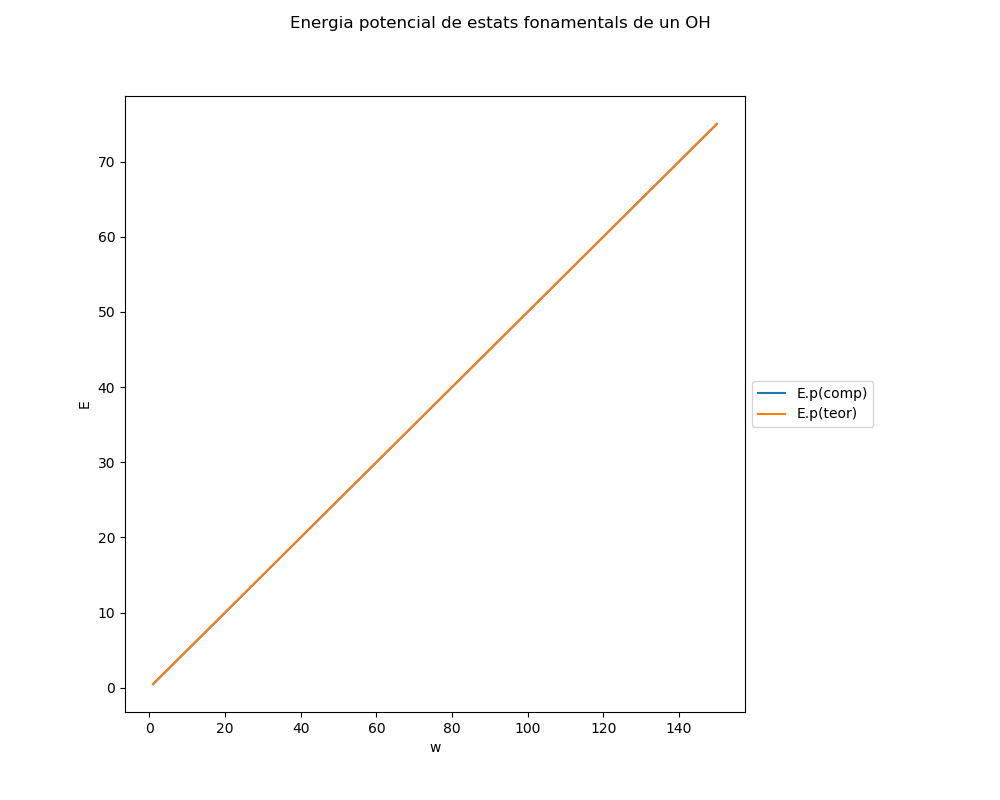
\includegraphics[width=\textwidth,height=7cm]{Epotharm.png}
\end{figure}
\begin{figure}[H]
	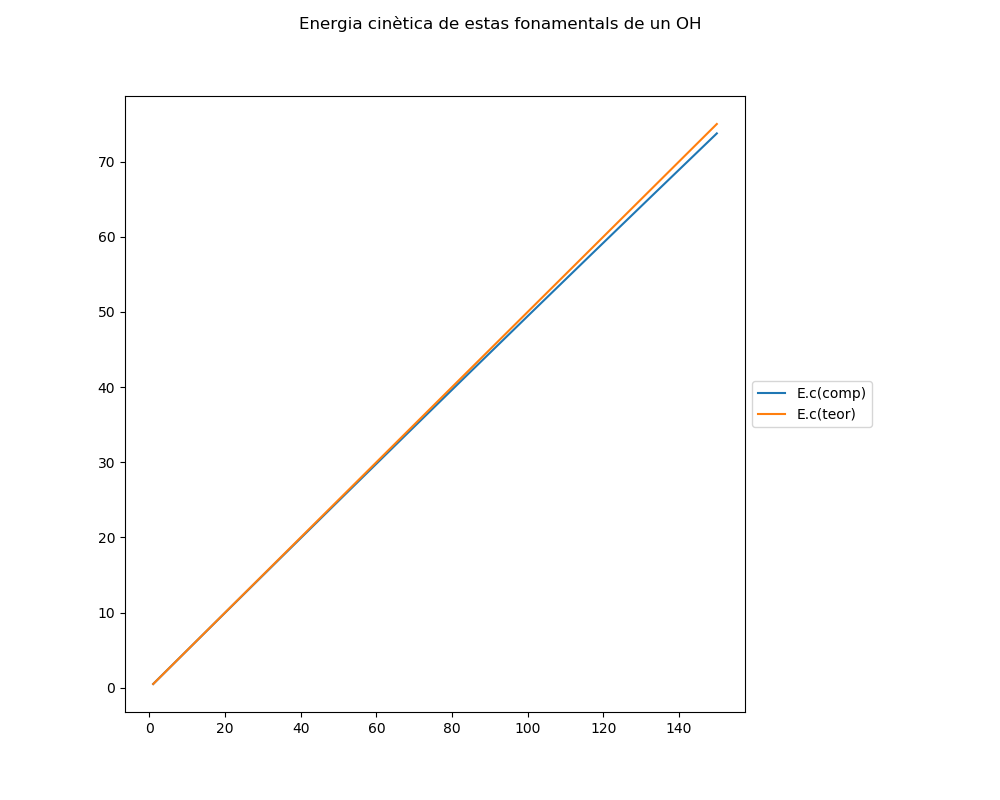
\includegraphics[width=\textwidth,height=7cm]{Ecinharm.png}
	\caption{Energia cinètica i potèncial de l'estat fonamental (\(n_x=0,n_y=0\)) de diversos oscil·ladors harmònic}
\end{figure}

Per tant, la manera de calcular la energia del paquet no pot ser cap error ja que es froça correcta. Llavors, vam fer evolucionar l'estat fonamental en un
cert temps t amb el mètode numèric, i vam obtenir una figura com aquesta:

\begin{figure}[H]
	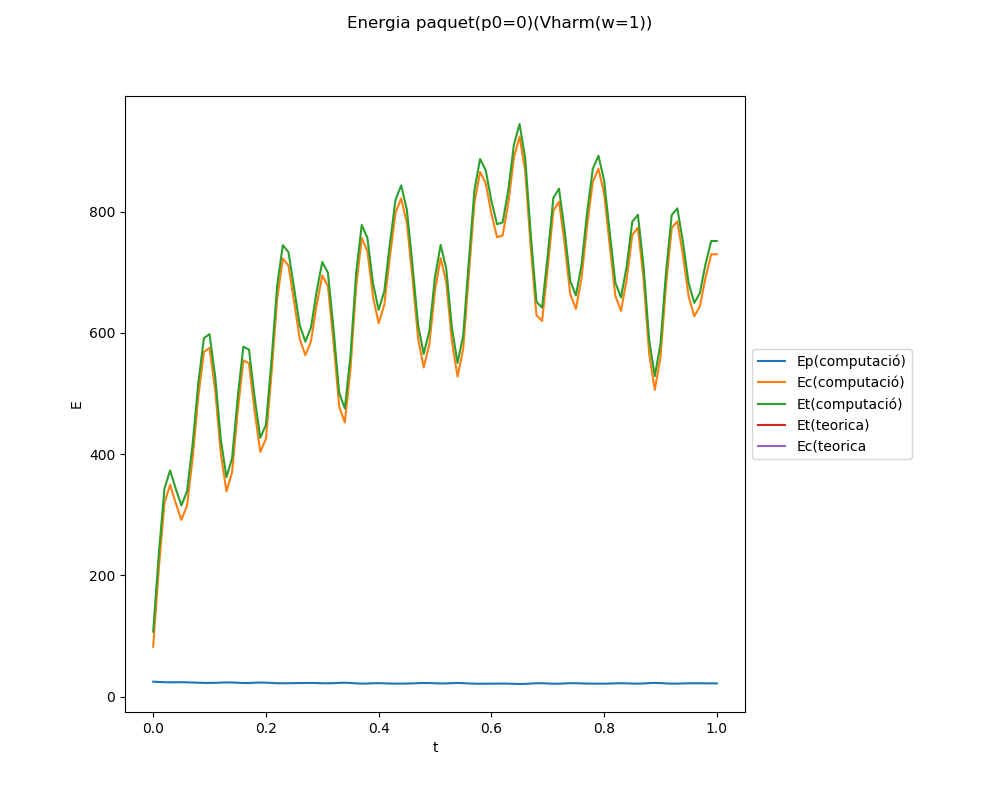
\includegraphics[width=\textwidth,height=7cm]{energiaharmdiscretitzat.png}
	\caption{Energia cinètica i potèncial de l'estat fonamental (\(n_x=0,n_y=0\)) de l'oscilador w=50 en diversos instants de t}
\end{figure}

Obviament, això estava malament, i vaig obtenir figures similars per tots els w. Per un altre banda, també estava obtenint un error en quant al valor esperat d'un paquet gaussià amb un p0=10, ja que no coincida amb el valor teòric. 

\begin{figure}[H]
	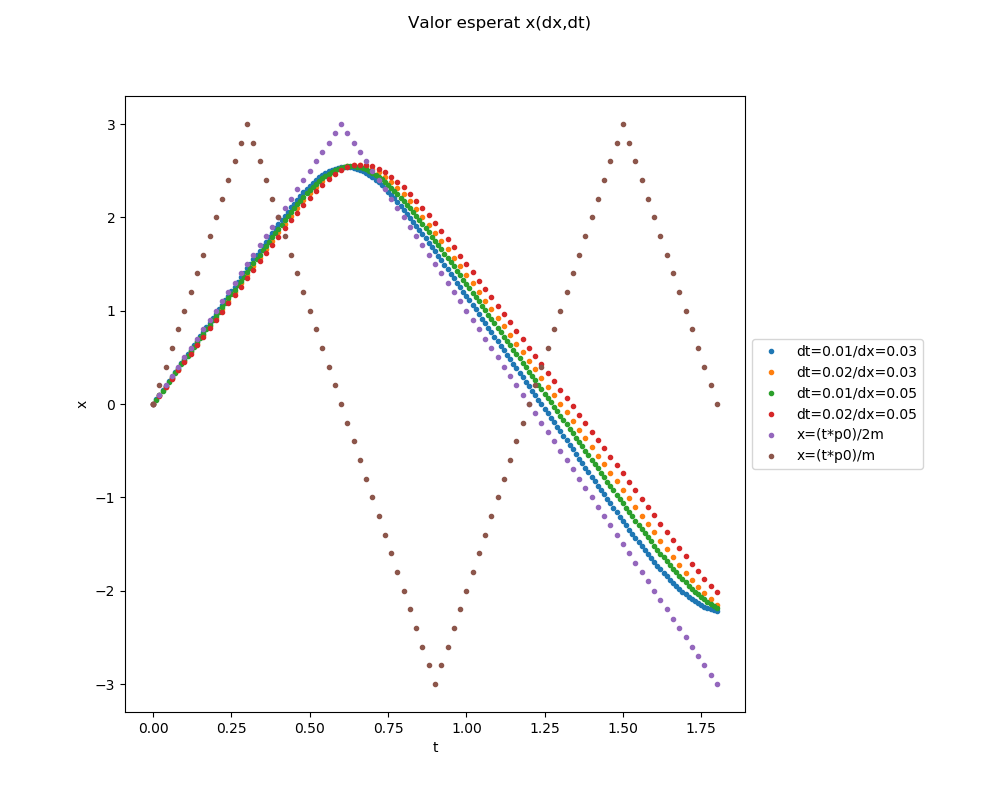
\includegraphics[width=\textwidth,height=7cm]{xespxmalament.png}
	\caption{Valor esperat del paquet i la seva predicció}
\end{figure}

Ja que el càlcul de la energia estava bé, l'error no podia provenir d'aquí. Així, em vaig posar a estudiar el problema amb el codi. El problema amb el valor esperat es solucionava afegint un factor 4 a la constant r, però no entenia perquè . Vaig rebuscar molt, i no vaig trobar cap error. Finalment, vaig pensar que tenia un problema conceptual amb el mètode en si. Llavors, rebuscant, resulta que em vaig equivocar a l'hora de plantejar el mètode i el vaig programar malament. El mètode es programa realment amb aquesta equació( on \(r=\frac{\Delta t \hbar}{4\Delta x^2 m}\)), que representa la primera iteració d'un pas:

\begin{align}
&\psi_{i,j}^{k+1/2}[1+(\frac{i\Delta t}{4\hbar}V_i+2r)]-r(\psi_{i+1,,j}^{k+1}+\psi_{i-1,j}^{k+1}) = \\
&\psi_{i,j}^{k}[1-(\frac{i\Delta t}{4\hbar}V_i+r)]+r(\psi_{i,j+1}^{k}+\psi_{i,j-1}^{k})
\end{align}

No obstant, el que jo estava fent era considerar en el membre de la dreta la mateixa derivada que en el de la esquerra, és a dir, estava aplicant un Crank-Nicolson 1D en cada fila, i despres en cada columna. En canvi, el mètode funciona de manera bastant diferent, com poden induïr de la equació anterior. Un cop trobat aquest error, vaig solucionar-ho, el que va implicar canviar el mètode i tornar a fer les comporvacions de conservació de norma i energia, valor esperat... Trobar l'error, modificar el mètode i tornar a comporvar que tot estava bé em van prendre bastant temps.

\section{Convergència del mètode}

Un cop solucionat l'error, vaig tornar a repetir els procediments anteriors, i vaig obtenir, aquest cop, solucions molt satisfactòries. Per un paquet gaussià de \(p_{ox}=5\) vam obtenir els següents resultats:

En quant al valor esperat, tenim que s'ha de satisfer:
\begin{equation}
<v>=\frac{<p>}{m}, \quad <X>=<v>t 
\end{equation}
Obtenim:
\begin{figure}[H]
	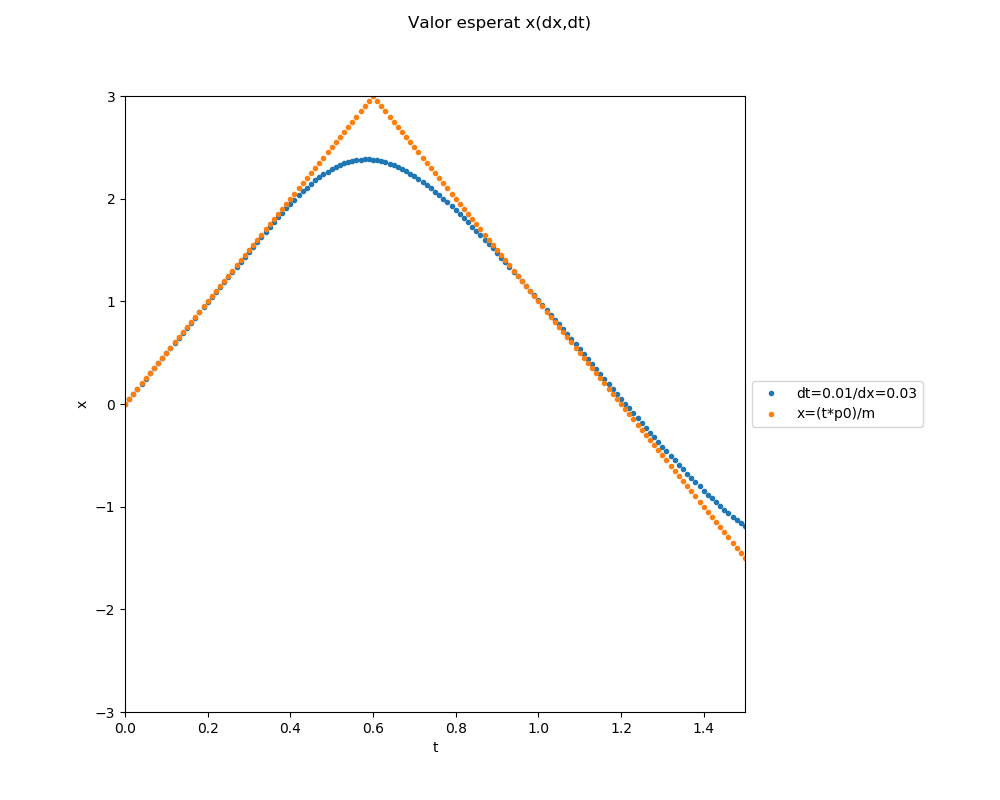
\includegraphics[width=\textwidth,height=7cm]{xespxp05dt0.png}
	\caption{Valor esperat del paquet de \(p_{ox}=5,p_{oy}=0\) i la seva predicció teòrica. Observem que coincideix bé el valor esperat teòric amb el calculat. }
\end{figure}

Per la dispersió en x i en y, tenim la següent equació analítca que s'ha de complir per un paquet gaussià lliure:
\begin{equation}
\sigma_x^2(t)=\sigma_x^2(0)+\frac{\sigma_p^2}{m^2}t^2, \quad \sigma_p^2=\frac{\hbar^2}{4\sigma_x(0)^2}
\end{equation}
El nostre paquet està tancat, però tot i així, aquesta equació és útil per fer una comparació en els instants inicials:
\begin{figure}[H]
	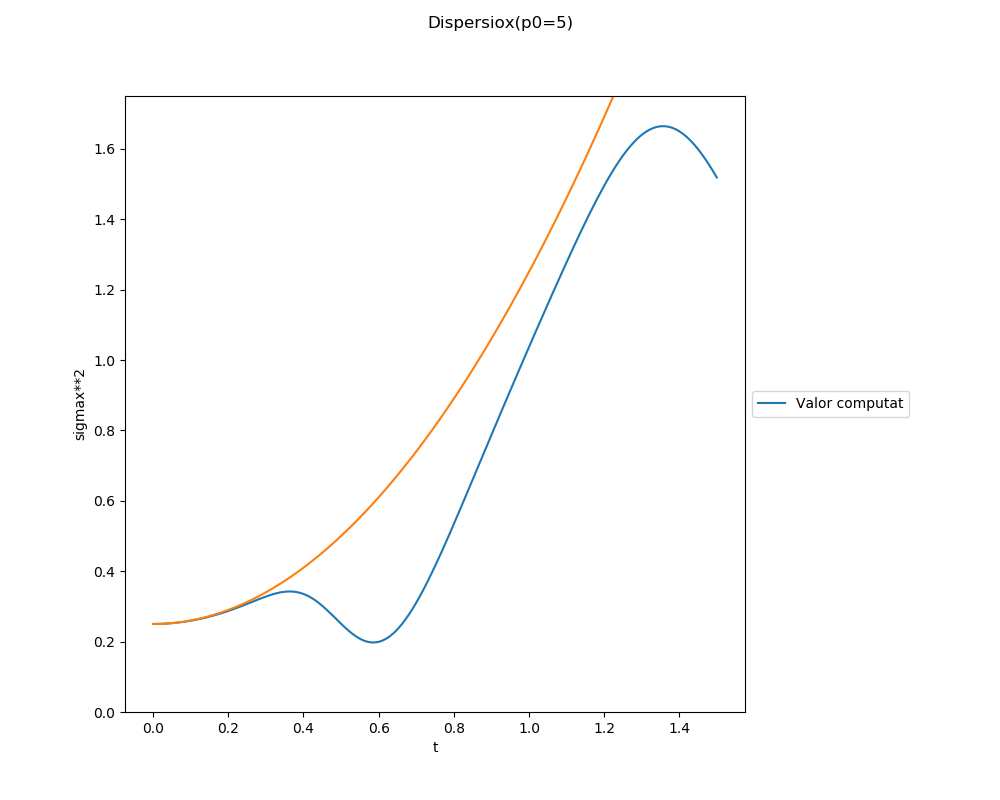
\includegraphics[width=\textwidth,height=7cm]{dispersioxpo5.png}
	\caption{Dispersio en x del paquet de \(p_{ox}=5,p_{oy}=0\) i la seva predicció teòrica. Observem que les dues funcions coincideixen bé inicialment. Posteriorment, ens trobem amb que el paquet xoca amb la paret, el que redueix repentinament la dispersió.}
\end{figure}
\begin{figure}[H]
	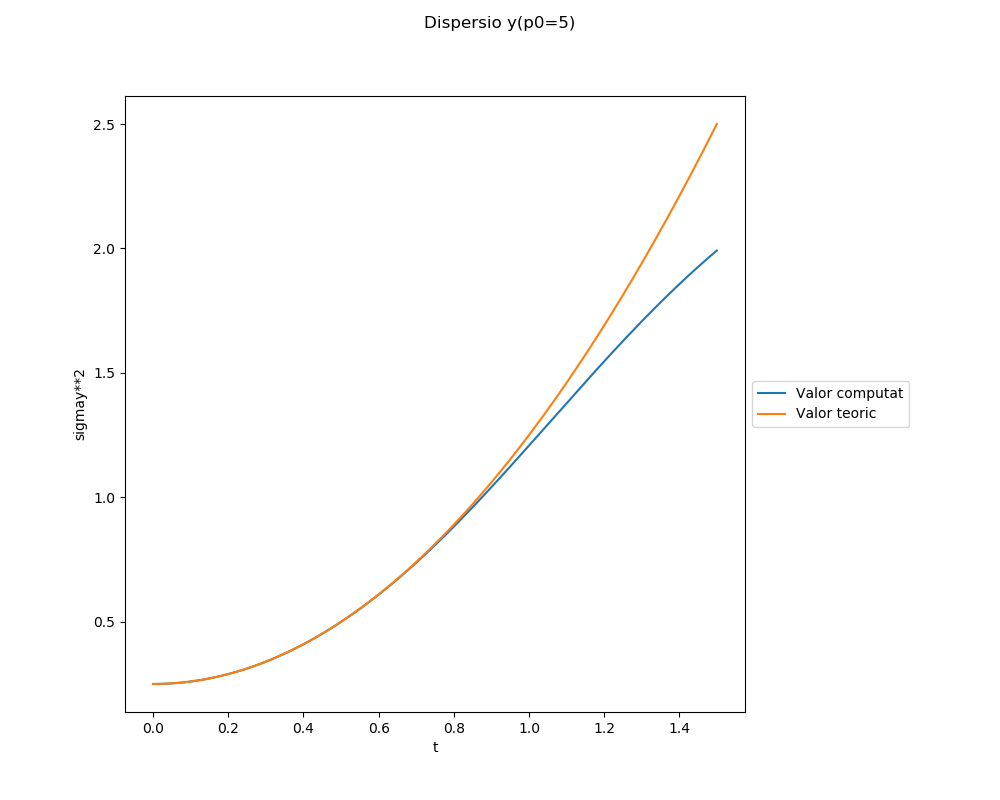
\includegraphics[width=\textwidth,height=7cm]{dispersioypo05.png}
	\caption{ Dispersio en y de \(p_{ox}=5,p_{oy}=0\) i la seva predicció teòrica. Observem que les dues funcions coincideixen bé durant un temps. Ja que no hi ha cap xoc amb les parets de \(y=\pm L\), les funcions coincideixen més temps que en la figura anterior.}
\end{figure}

Finalment, vam tornar a aplicar el problema de l'oscilador harmonic i vam obtenir les següents figures:

\begin{figure}[H]
	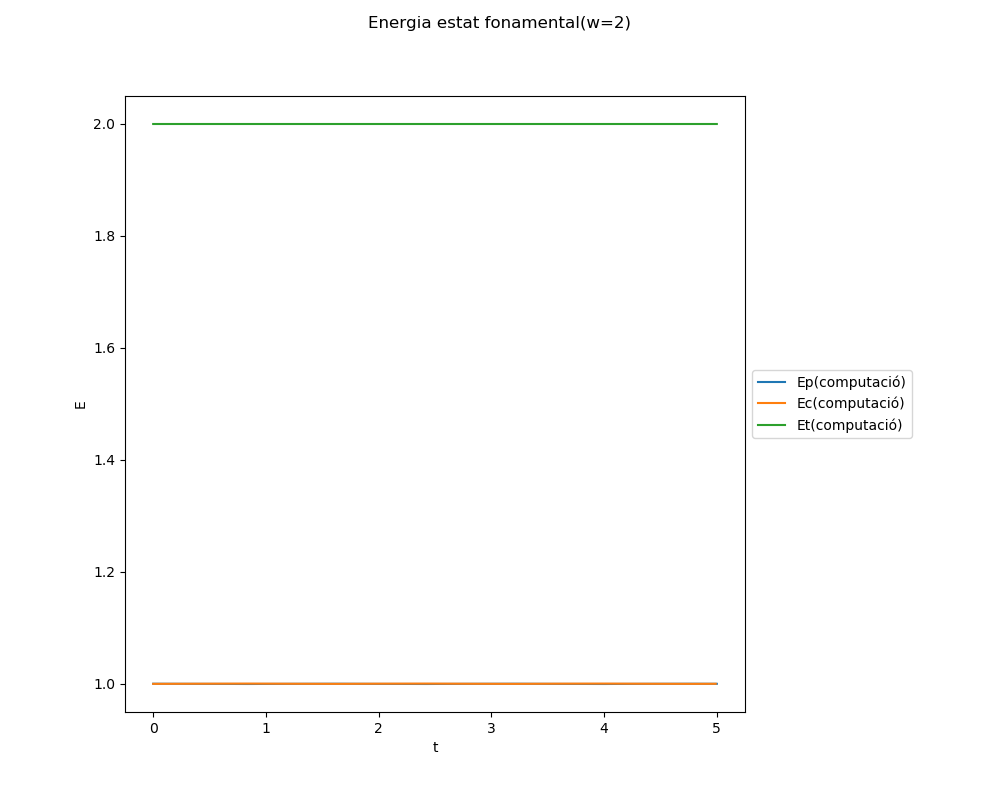
\includegraphics[width=\textwidth,height=8cm]{Eharm2.png}
	\caption{Energia potèncial de l'estat fonamental (\(n_x=0,n_y=0\)) de l'oscilador w=2 en diversos instants de t}
\end{figure}
\begin{figure}[H]
	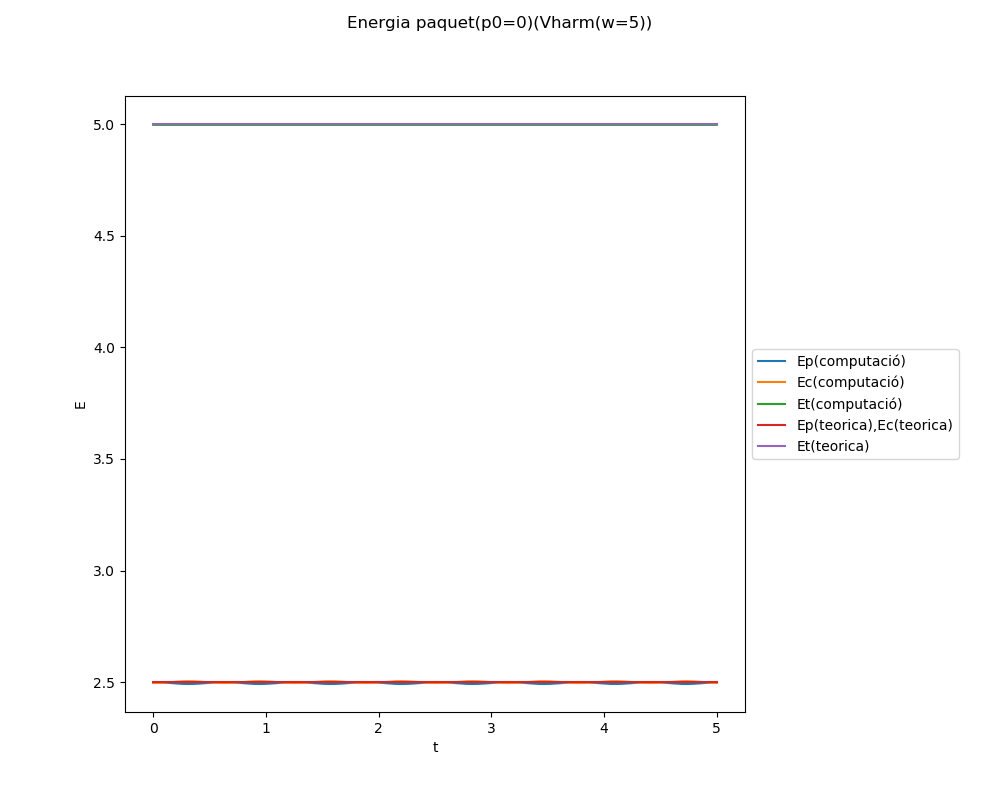
\includegraphics[width=\textwidth,height=8cm]{Eharmpot3.png}
	\caption{Energia potèncial de l'estat fonamental (\(n_x=0,n_y=0\)) de l'oscilador w=5 en diversos instants de t}
\end{figure}
\begin{figure}[H]
	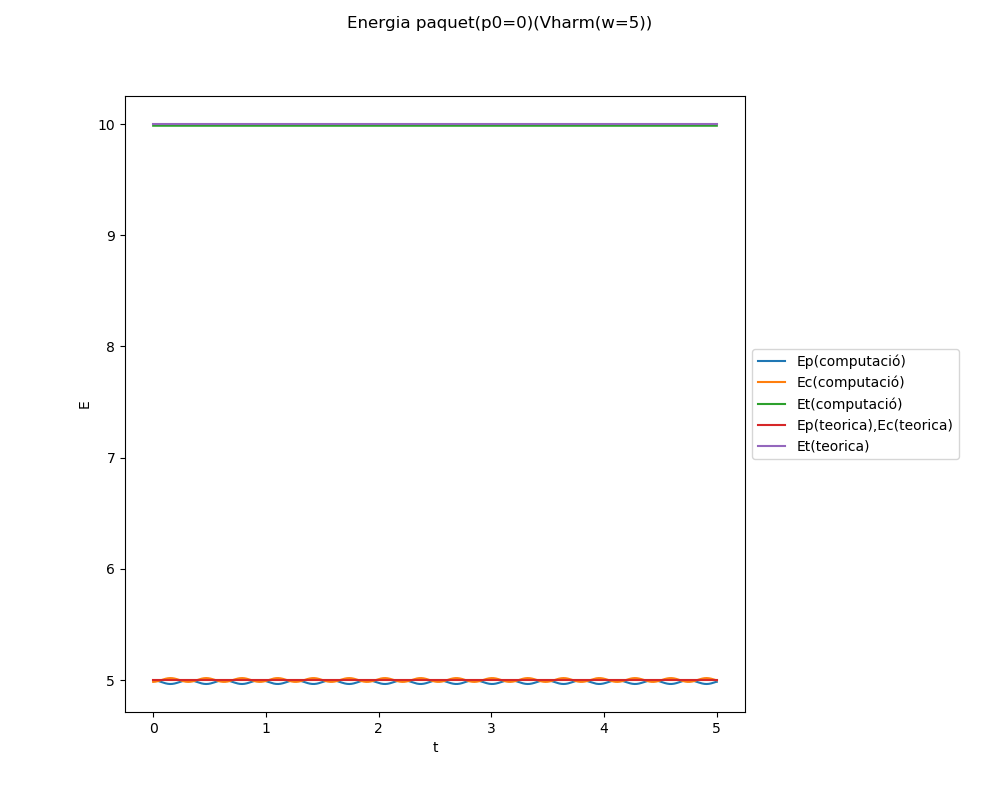
\includegraphics[width=\textwidth,height=8cm]{Eharmpot4.png}
	\caption{Energia potèncial de l'estat fonamental (\(n_x=0,n_y=0\)) de l'oscilador w=10 en diversos instants de t}
\end{figure}

Per tant, podem confrimar que el mètode convergeix força bé.



\end{document}
